\documentclass[11pt]{article}
\usepackage{amsmath}
\usepackage{tikz}

\usetikzlibrary{arrows,shapes,pgfplots.groupplots,positioning}
\tikzset{dots/.style={dash pattern = on 1pt off 1pt}}
\tikzset{pointille/.style={dash pattern = on 1pt off 2pt on 3pt off 2pt}}
\tikzset{tirets/.style={dash pattern = on 5pt off 5pt}}

\newcommand{\vecttheta}{\mbox{\boldmath{$\theta$}}}
\newcommand{\thetaOpt}{\ensuremath{\vecttheta^{*}}}

\begin{document}
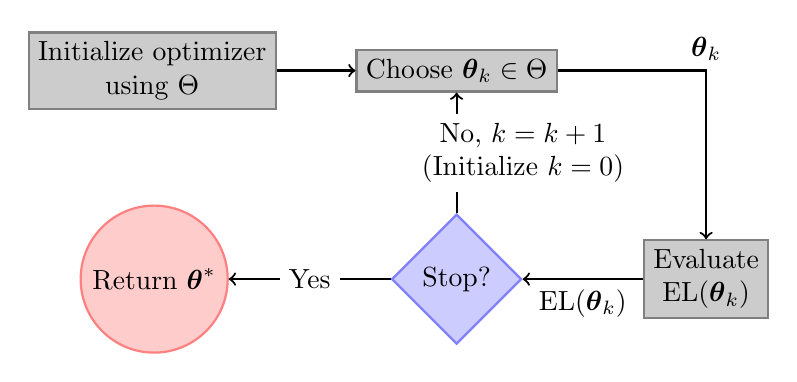
\begin{tikzpicture}[
  action/.style={rectangle,draw=black!50,fill=black!20,thick},
  endpoint/.style={circle,draw=red!50,fill=red!20,thick},
  question/.style={diamond,draw=blue!50,fill=blue!20,thick},
  align=center]

  \node[question] (stop) {Stop?};
  \node[action] (ask) [above=of stop, yshift=3.5ex] {Choose $\vecttheta_{k}\in\Theta$};
  \node[action] (evaluate loss function) [right=of stop, xshift=1.5em] {Evaluate\\$\text{EL}(\vecttheta_{k})$};

  \node[endpoint] (best) [left=of stop, xshift=-3em] {Return $\thetaOpt$};
  \node[action] (start) [above=of best, left=of ask] {Initialize optimizer\\using $\Theta$};

  \draw[->,thick] (start) -- (ask);
  \draw[->,thick] (ask) -| node[above, midway] {$\vecttheta_{k}$} (evaluate loss function);
  \draw[->,thick] (evaluate loss function) -- node[below, midway] {$\text{EL}(\vecttheta_{k})$} (stop);
  \draw[->,thick] (stop) -- node[xshift=2.4em, fill=white] {No, $k = k+1$\\(Initialize $k=0$)} (ask);
  \draw[->,thick] (stop) -- node[midway, fill=white] {Yes} (best);
\end{tikzpicture}
\end{document}